\section{Exemple: un calcul de propagation avec \freefem}

\medskip
Quelque soit le logiciel utilisé\footnote{%
Lorsque l'on parle de codes éléments finis, on cite les grands noms du domaine... et ils correspondent à des
codes extraordinairement puissants, mais souvent chers.

Or un certain nombre de codes éléments finis professionnels sont disponibles gratuitement (au téléchargement
et à l'utilisation).
Les deux plus connus sont \castem (anciennement castem) et \aster développés et maintenus
par le CEA et par EDF respectivement.%
}, il y a toujours un gros pavé d'exemple fourni avec,
sans compter le nombre d'ouvrages disponibles.

\medskip
Nous avons souhaité néanmoins présenter un listing (qui sera discuté oralement)
correspondant à un calcul réalisé sous \freefem.

Ce logiciel gratuit vous permettra de faire vos calculs EF... mais c'est également un outil 
pédagogique sans équivalent: sa manipulation se fait en des termes proches de la
formulation mathématique, et en cela, il est une passerelle parfaite entre la théorie
et la pratique de codes plus «industriels».

Le fait de pouvoir discrétiser à loisir une formulation variationnelle que l'on rentre
soi-même est également un argument qui nous semble un vrai plus, même si
cela commence à exister dans des codes commerciaux (mais reste confidentiel).

\medskip
Voici donc un petit listing sur lequel nous pourrons revenir de vive voix.
%Je ne vous dis même pas de quoi il s'agit...

Commençons donc, comme il se doit, par définir la géométrie du problème, paramétrée
par~$a$ et~$b$, que nous maillons:

\medskip
\color{gris}\scriptsize
%\begin{multicols}{2}
\begin{Verbatim}[numbers=left,numbersep=3pt]
real mu=1.; 
real rog=0. , ro=1.;
// taille du maillage
int ncuts = 20;

// construction du domaine
real a=pi*0.8, b=1.2*pi ; 

border gam1(t=0.,a){x=t;y=0; label =1;};
border gam2(t=0.,b){x=a;y=t; label =2;};
border gam3(t=a,0.){x=t;y=b; label =3;};
border gam4(t=b,0.){x=0.;y=t; label =4;};

//Maillage
mesh Th=buildmesh(gam1(ncuts)+gam2(ncuts)+gam3(ncuts)+gam4(ncuts)); 
//plot(Th, ps="mesh.eps") ;
//plot(Th, wait=1) ;
\end{Verbatim}
%\end{multicols}
\color{black}\normalsize

\medskip
Nous définissons quelques valeurs afin de pouvoir définir le chargement (dont l'un des chargement,
défini par la fonction~$w_1$ ne sera pas utilisée dans la suite). Notons comme il est aisé de définir
des fonctions:

\color{gris}\scriptsize
\begin{multicols}{2}
\begin{Verbatim}[numbers=left,numbersep=3pt,firstnumber=last]
// conditions aux limites essentielles 
real r0=a/10., r, xc=a/3., yc=3.*b/4.; 

// chargement initial sinusoidal
func real pertb(real r)
	{ if(r<r0) {return (1.+cos(pi*r/r0));}
	else return 0.;}

//func real w1( real x, real y)
func real w11( real x, real y)
{
	return pertb(sqrt((x-xc)^2+(y-yc)^2)); 
}

// chargement constant sur un carre
// pas utilise sur cet exemple
func real w1( real c, real d)
{
 if(c>(0.8*xc))
   {if (c<(1.2*xc)) 
    {if (d>(0.8*yc))
      {if (d<(1.2*yc)) {return 0.8;}
      else return 0.;}
    else return 0.;}
   else return 0.;}
	else return 0.;
}

func real w0( real x, real y)
{
	return 0.*sin(x)*sin(y) ; 
}
\end{Verbatim}
\end{multicols}
\color{black}\normalsize

\medskip
Ensuite, nous définissons l'espace des éléments finis utilisés, et les variables appartenant à ces espaces.
L'analogie avec la «formulation mathématique» saute au yeux... et c'est pourquoi cet outil
nous semble particulièrement intéressant sur le plan pédagogique.

\color{gris}\scriptsize
%\begin{multicols}{2}
\begin{Verbatim}[numbers=left,numbersep=3pt,firstnumber=last]
// Espaces elements finis 
fespace Vh(Th,P2); 
fespace Wh(Th,P1dc);

Vh w, wa, wd, wda, wdd, wdda, fi ; 
Wh sxz, syz ; 
\end{Verbatim}
%\end{multicols}
\color{black}\normalsize

\medskip
Il s'agit d'un exemple non stationnaire, nous allons donc faire une boucle sur le temps. 
Dans \freefem, nous entrons directement la formulation variationnelle du problème sous forme «mathématique»... 
le lien entre pratique des éléments finis et théorie est beaucoup plus clair. 
La boucle de temps est basée sur un schéma de Newmark implicite. Le temps «courant»
est le temps~$t+\Delta_t$ et le temps précédent est le temps~$t$ pour rester cohérent avec
les notations du chapitre~\ref{Ch-temps}.

Il s'agit d'un problème de déplacement hors plan, dont le champ inconnu est traditionnellement
noté~$w$. Ainsi, dans le listing, \verb|w| représente~$q_{t+\Delta_t}$, \verb|wa|$\equiv q_t$, 
\verb|wd|$\equiv \dot{q}_{t+\Delta_t}$, \verb|wda|$\equiv \dot{q}_t$, 
\verb|wdd|$\equiv \ddot{q}_{t+\Delta_t}$ et \verb|wdda|$\equiv \ddot{q}_t$. \verb|fi|$\equiv\varphi$
est la fonction test. La formulation variationnelle, en n'indiçant pas le temps actuel et en utilisant l'indice~$a$
pour le pas de temps précédent ($a$ comme avant), est:
\begin{equation}
\begin{array}{rl}
\text{antiplane}(\dot{w},\varphi) = &
	\dint_{Th} \rho \dot{w} \varphi + 
		\frac{\Delta_t^2}4 \dint_{Th} \mu \left( \dfrac{\partial \dot{w}}{\partial x}\dfrac{\partial \varphi}{\partial x} +
		\dfrac{\partial \dot{w}}{\partial y}\dfrac{\partial \varphi}{\partial y}\right)\\[+3ex]
	& - 	\dfrac{\Delta_t}2 \dint_{Th} \rho_g \varphi 
	- \dint_{Th} \rho\left(\dot{w}_a+\frac{\Delta_t}2 \ddot{w}_a\right)\varphi \\[+3ex]
	& + \dfrac{\Delta_t}2 \dint_{Th} \mu \left( \dfrac{\partial w_a}{\partial x}\dfrac{\partial \varphi}{\partial x}
		+ \dfrac{\partial w_a}{\partial y}\dfrac{\partial \varphi}{\partial y} \right) \\[+3ex]
	& + \dfrac{\Delta_t^2}4 \dint_{Th} \mu \left( \dfrac{\partial \dot{w}_a}{\partial x}\dfrac{\partial \varphi}{\partial x} +
		\dfrac{\partial \dot{w}_a}{\partial y}\dfrac{\partial \varphi}{\partial y} \right) \\[+3ex]
	& + \text{Condition } (\dot{w}=0 \text{ sur les lignes } 1,2,3,4)
\end{array}
\end{equation}

\color{gris}\scriptsize
%\begin{multicols}{2}
\begin{Verbatim}[numbers=left,numbersep=3pt,firstnumber=last]
int n, k, Ntemps=100; 
real T=2.*pi/sqrt(2.), pastemps=T/Ntemps
real dpt=0.5*pastemps; 

problem antiplane(wd,fi, init=1)=int2d(Th)(ro*wd*fi)+ 
		int2d(Th)(dpt^2*mu*(dx(wd)*dx(fi)+dy(wd)*dy(fi))) + 
		int2d(Th)(-dpt*rog*fi)+
		int2d(Th)(ro*(-wda-dpt*wdda)*fi)+
		int2d(Th)(dpt*mu*(dx(wa)*dx(fi)+dpt*dx(wda)*dx(fi)+
		dy(wa)*dy(fi)+dpt*dy(wda)*dy(fi)))+
		on(1,2,3,4,wd=0.); 

// formulation du probleme en temps
// conditions initiales en temps
w=w0(x,y);
wd=w11(x,y); 
wdd=0.; 

real errorw, errorwd, temps, enerC, enerP, enerT; 
real[int] visoS(20);
int ivi; 
for (ivi=0;ivi<10;ivi++){
	visoS[ivi]=-1+0.1*ivi;
	visoS[ivi+10]=(ivi+1)*0.1;
}
\end{Verbatim}
%\end{multicols}
\color{black}\normalsize

\medskip
Enfin, pour tester la qualité des résultats, il nous faut quelques indicateurs...
Sans entrer dans le détail, des noms comme~$E_c$, $E_p$ et~$E_T$ doivent vous mettre sur
la piste.

\color{gris}\scriptsize
%\begin{multicols}{2}
\begin{Verbatim}[numbers=left,numbersep=3pt,firstnumber=last]
real[int] Ec(Ntemps), Ep(Ntemps), Et(Ntemps), tt(Ntemps); 

for (n=0;n<Ntemps;n++){	
	wa=w; wda=wd; wdda=wdd; 	
	temps=n*pastemps; 

	enerC=0.5*int2d(Th)(ro*wd^2);
	enerP=0.5*int2d(Th)(mu*(dx(w)*dx(w)+ dy(w)*dy(w)));
	enerT=enerC+enerP;
	Ec(n)=enerC; Ep(n)=enerP; Et(n)=enerT; tt(n)=temps; 
		
	cout << " iteration n= " << n << " enerP= " << enerP << 
    "enerC= " << enerC << " enerTotale= " << enerT 
     << endl;
	
	temps=(n+1.)*pastemps; 

// resolution du probleme 
	antiplane;
	
	w=wa+dpt*(wda+wd);
	wdd=(wd-wda)/dpt-wdda; 

	sxz=mu*dx(w);
	syz=mu*dy(w); 
	plot(Th,wd,fill=true, value=1, viso=visoS, nbiso=visoS.n, 
     ps=n, wait=0); 	
}

// Energie 
//plot([tt,Ec], [tt,Ep],[tt,Et], ps="energie.eps"); 
\end{Verbatim}
%\end{multicols}
\color{black}\normalsize

\medskip
À la \fig{Fig-Exo6} se trouve une illustration de ce que nous venons de calculer.

\begin{figure}[ht]
  \center
  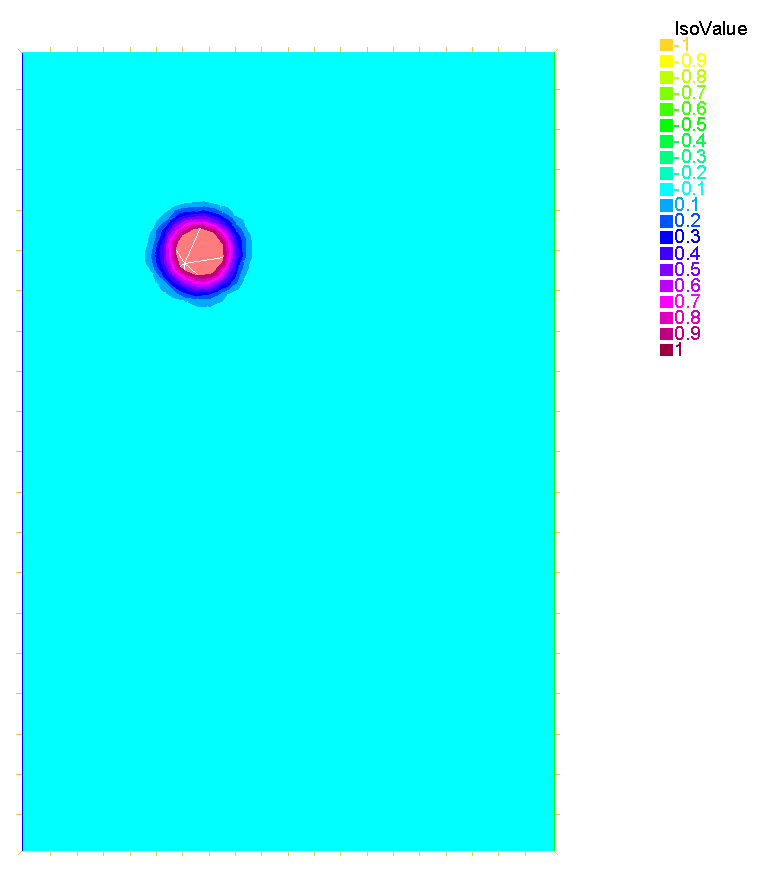
\includegraphics[height=55mm]{Exo6pas00.eps} \hfill
  \includegraphics[height=55mm]{Exo6pas20.eps} \hfill
  \includegraphics[height=55mm]{Exo6pas40.eps}
  \caption{\label{Fig-Exo6} Propagation: pas de temps 0, 20 et 40}
\end{figure}

